\let\negmedspace\undefined
\let\negthickspace\undefined
\documentclass[journal]{IEEEtran}
\usepackage[a5paper, margin=10mm, onecolumn]{geometry}
%\usepackage{lmodern} % Ensure lmodern is loaded for pdflatex
\usepackage{tfrupee} % Include tfrupee package

\setlength{\headheight}{1cm} % Set the height of the header box
\setlength{\headsep}{0mm}     % Set the distance between the header box and the top of the text

\usepackage{gvv-book}
%\usepackage{gvv}
\usepackage{cite}
\usepackage{amsmath,amssymb,amsfonts,amsthm}
\usepackage{algorithmic}
\usepackage{graphicx}
\usepackage{textcomp}
\usepackage{xcolor}
\usepackage{txfonts}
\usepackage{listings}
\usepackage{enumitem}
\usepackage{mathtools}
\usepackage{gensymb}
\usepackage{comment}
\usepackage[breaklinks=true]{hyperref}
\usepackage{tkz-euclide} 
\usepackage{listings}
\usepackage{gvv}                                        
\def\inputGnumericTable{}                                 
\usepackage[latin1]{inputenc}                                
\usepackage{color}                                            
\usepackage{array}                                            
\usepackage{longtable}                                       
\usepackage{calc}                                             
\usepackage{multirow}                                         
\usepackage{hhline}                                           
\usepackage{ifthen}                                           
\usepackage{lscape}
\begin{document}

\bibliographystyle{IEEEtran}

\title{2.10.48}
\author{EE25BTECH11019 - Darji Vivek M.}
{\let\newpage\relax\maketitle}

\renewcommand{\thefigure}{\theenumi}
\renewcommand{\thetable}{\theenumi}
\setlength{\intextsep}{10pt}
\numberwithin{figure}{enumi}
\renewcommand{\thetable}{\theenumi}

\textbf{Question}:\\
If $\vec{a} = \vec{i}+\vec{j}+\vec{k}$, $\vec{a}\cdot\vec{b}=1$ and $\vec{a}\times\vec{b}=\vec{j}-\vec{k}$, then $\vec{b}$ is  

\begin{multicols}{2}
\begin{enumerate}[label=(\alph*)]
\item $\vec{i}-\vec{j}+\vec{k}$  
\item $2\vec{j}-\vec{k}$  
\item $\vec{i}$  
\item $2\vec{i}$  
\end{enumerate}
\end{multicols}  

\solution  

\begin{align}
\vec{a} &= \myvec{1\\1\\1}, \quad 
\vec{b} = \myvec{x\\y\\z}
\end{align}

Dot product condition:
\begin{align}
\myvec{1 & 1 & 1}\myvec{x\\y\\z}=1
\end{align}

Cross product condition gives
\begin{align}
\myvec{0 & 1 & -1}\myvec{x\\y\\z}=0
\end{align}

Collecting all equations:
\begin{align}
\myvec{0 & 1 & -1\\ 1 & 0 & -1\\ 1 & 1 & 1}\myvec{x\\y\\z}=\myvec{0\\1\\1}
\end{align}

Solving,
\begin{align}
\myvec{x\\y\\z}=\myvec{1\\0\\0}
\end{align}

Hence,
\begin{align}
\vec{b}=\myvec{1\\0\\0}=\vec{i}
\end{align}

Therefore, the correct option is (c).

\begin{figure}[H]
\centering
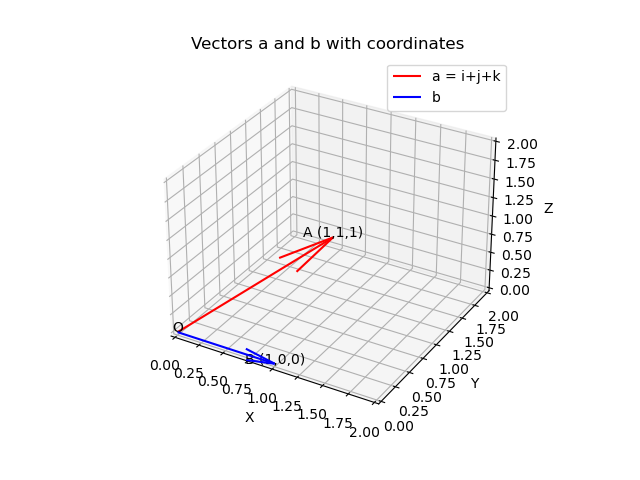
\includegraphics[width=0.75\columnwidth]{figs/5.png}
\caption{\centering plot}
\label{fig:placeholder_125}
\end{figure}
\end{document}
